
\begin{figure}
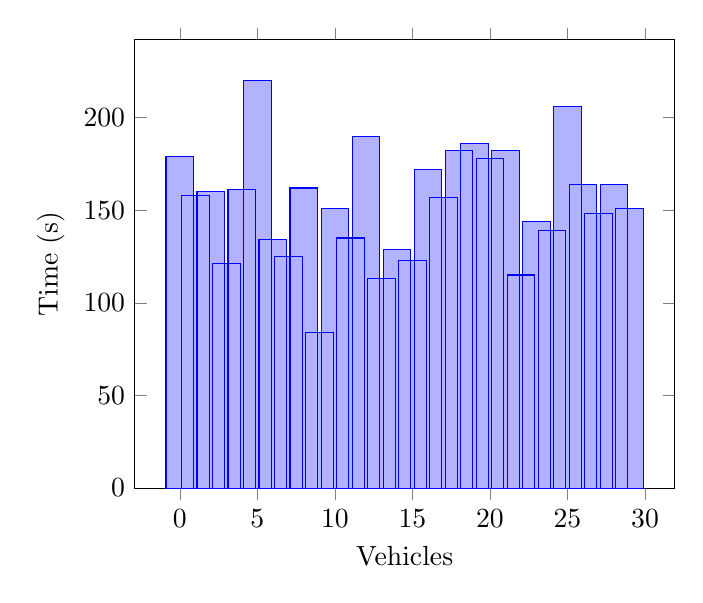
\begin{tikzpicture}
\begin{axis}[
legend style={anchor=west},
xlabel=Vehicles,
ylabel=Time (s),
ymin=0,
ybar,
]
\addplot coordinates {
(0, 179)
(1, 158)
(2, 160)
(3, 121)
(4, 161)
(5, 220)
(6, 134)
(7, 125)
(8, 162)
(9, 84)
(10, 151)
(11, 135)
(12, 190)
(13, 113)
(14, 129)
(15, 123)
(16, 172)
(17, 157)
(18, 182)
(19, 186)
(20, 178)
(21, 182)
(22, 115)
(23, 144)
(24, 139)
(25, 206)
(26, 164)
(27, 148)
(28, 164)
(29, 151)
};

\end{axis}
\end{tikzpicture}
\label{tik:0:19_O, 19_O.-60, 17_N, 15_S, 15_S.-30, 13_N, 13_N.-40, 11_N, 8_N, 7_N, 7_N.-60, 5_N, 4_N, 4_N.-60, 1_N}
\caption{0 percent diving with GSC on route $19_O, 19_O.-60, 17_N, 15_S, 15_S.-30, 13_N, 13_N.-40, 11_N, 8_N, 7_N, 7_N.-60, 5_N, 4_N, 4_N.-60, 1_N$}
\end{figure}
